% Created with jtex v.1.0.4
%%%%%%%%%%%%%%%%%%%%%%%%%%%%%%%%%%%%%%%%%%%%%%%%%%%%%%%%%%%%
%%% LaPreprint: PREPRINT TEMPLATE
%%%%%%%%%%%%%%%%%%%%%%%%%%%%%%%%%%%%%%%%%%%%%%%%%%%%%%%%%%%%

% Here I could talk about what one should do in this document.
% Instead I'll refer you to the explore on your own and check the Github Repo. :-)
% Line spacing is 1.2 by default (can't be smaller).

%%%%%%%%%%%%%%%%%%%%%%%%%%%%%%%%%%%%%%%%%%%%%%%%%%%%%%%%%%%%
%%% PREAMBLE
%%%%%%%%%%%%%%%%%%%%%%%%%%%%%%%%%%%%%%%%%%%%%%%%%%%%%%%%%%%%

% Declare document class
\documentclass[9pt,Preprint]{lapreprint}
% Choose between "biorxiv", "medrxiv", "arxiv" and "chemrxiv". Otherwise defaults "Preprint".
% Choose between "blue" and "red" colour scheme. Defaults to "blue".
% Use the "onehalfspacing" option for 1.5 line spacing.
% Use the "doublespacing" option for 2.0 line spacing.
% Use the "lineno" option for line numbers.
% Use the "endfloat" option to place floats after the bibliography.
% Use the "secnum" option to have include numbers.

% Import packages
% \usepackage{lipsum}     % Required to insert dummy text
\usepackage[version=4]{mhchem} % For chemical notation
\usepackage{siunitx}    % For SI units
\usepackage{pdflscape}  % For putting pages in landscape mode
\usepackage{rotating}   % For rotating specific elements
\usepackage{textgreek}  % Greek symbols
\usepackage{gensymb}    % Symbols
\usepackage[misc]{ifsym} % For the \Letter symbol
\usepackage{orcidlink}  % For the \orcidlink
\usepackage{listings}   % For inserting code chunks
\usepackage{colortbl}   % For Knitr table colouring
\usepackage{tabularx}   % For making Knitr tables compatible
\usepackage{longtable}  % For multi-page tables
\usepackage{subcaption}
\usepackage{multirow}
\usepackage{snotez}     % For sidenote environments. enotez for endnotes
\usepackage{csquotes}   % For language-based quote rules (helps BiBLaTeX)



% Make declarations
\DeclareSIUnit\Molar{M}

% Please note that these options may affect formatting.

%%%%%%%%%%%%%%%%%%%%%%%%%%%%%%%%%%%%%%%%%%%%%%%%%%%%%%%%%%%%
%%% BIBLIOGRAPHY
%%%%%%%%%%%%%%%%%%%%%%%%%%%%%%%%%%%%%%%%%%%%%%%%%%%%%%%%%%%%
\usepackage[			% use biblatex for bibliography
	backend=biber,      % use biber or bibtex backend
    style=authoryear,   % choose style
	natbib=true,		% allow natbib commands
	hyperref=true,	    % activate hyperref support
	alldates=year,      % only show year (not month)
]{biblatex}

% Just avoiding some rogue fields that cause issues with certain styles
\AtEveryBibitem{
    \clearfield{urlyear}
    \clearfield{urlmonth}
    \clearlist{language}
}

% Update to your bibliography file
\addbibresource{main.bib}


%%%%%%%%%%%%%%%%%%%%%%%%%%%%%%%%%%%%%%%%%%%%%%%%%%%%%%%%%%%%
%%% ARTICLE SETUP
%%%%%%%%%%%%%%%%%%%%%%%%%%%%%%%%%%%%%%%%%%%%%%%%%%%%%%%%%%%%

% Paper title
\title{History and Background}

% Authors - you can use \orcidlink{} and \authfn{} - see contribution note
\author[1]{Paul Skrzypczyk}

% Affiliations
\affil[1]{School of Physics, University of Bristol}

% Other metadata. Feel free to add your own
\metadata[]{Keywords}{}


% Surname of the lead author(s) for the running footer
\leadauthor{Paul Skrzypczyk}
\shorttitle{History}

%%%%%%%%%%%%%%%%%%%%%%%%%%%%%%%%%%%%%%%%%%%%%%%%%%%%%%%%%%%%
%%% ARTICLE START
%%%%%%%%%%%%%%%%%%%%%%%%%%%%%%%%%%%%%%%%%%%%%%%%%%%%%%%%%%%%

\begin{document}
\maketitle


Quantum mechanics constitutes a huge departure from classical physics and completely alters the view we have of how the universe functions. In order to understand where quantum mechanics came from, and why it was necessary to replace classical physics by it, in this first section we briefly describe some of the key phenomena that arose, roughly around the turn of the last century, that classical physics was simply unable to give a satisfactory explanation of. The list here will be neither comprehensive nor in chronological order, but is meant just to provide a short account of the main difficulties faced by classical physics, for which a new physical theory was ultimately necessary. We will also discuss at the same time some of the early ideas and insights which would eventually develop into the theory that we now call quantum mechanics. The goal of this section is to set the scene and provide the a small amount of context for the following sections, where we will begin our exploration of quantum mechanics.

\subsection{The photoelectric effect}\label{The photoelectric effect}

A key effect that classical physics was unable to explain is the \textbf{photoelectric effect}. It is observed that if light is shone on a piece of metal, then electrons are emitted. This effect can be studied carefully by forming a capacitor out of two metal plates in vacuum, placing this in a circuit, and applying a voltage (potential difference) across the plates.

\begin{figure}[!htbp]
\centering

\includegraphics[width=0.625\linewidth]{files/photoelectric-825d7eb67bd367836564ff4360164029.svg}
\caption[]{\textbf{The photoelectric effect.} Schematic diagram of the photoelectric effect. Light of a fixed frequency $f$ is shone on one of the metal plates of a capacitor (which is in a vacuum). This causes electrons to be emitted. Some of these arrive at the other place, and a current is generated. By placing a potential across the plates the maximum kinetic energy of the emitted electrons can be measured.}
\label{photoelectric}
\end{figure}

When light is shone on one of the plates, it causes a current to flow, which is how we know that electrons are being emitted. Varying the potential difference between the plates allows us to study the \textbf{kinetic energy} of the emitted electrons. It is observed that if light of a \textbf{fixed wavelength} $\lambda$, and therefore frequency $f = c\lambda$, is shone, then for all metals the maximum kinetic energy $E_\mathrm{max}$ of the electrons emitted follows a simple rule

\begin{equation}
E_\mathrm{max} = h f - \phi,
\end{equation}

where $h$ is a constant of nature known as Planck's constant (since it was discovered by Planck, while exploring blackbody radiation), and equal to

and $\phi$ is known as the \textbf{workfunction}, and is in general different for different metals. This maximum energy is determined by shining the light on the plate at the lower potential, and measuring the potential difference that needs to be put between the plates in order to \textbf{just stop} the current, since in order to reach the other plate (and generate a current) the electron needs enough kinetic energy to overcome this potential difference.

There are some particularly surprising aspects about what is observed:

\begin{itemize}
\item As the \textbf{intensity} of light is increased, the \textbf{rate} at which electrons are emitted increases -- producing a bigger current -- but does \textbf{not} affect the maximum energy of the emitted photons, as measured by varying the potential.
\item Even for extremely weak light, a small current is observed to begin flowing \textbf{immediately} when the light is shone on the metal. That is, there is no delay after shining the light before some current starts flowing.
\item Low frequency/long wavelength light, for example red light, for certain metals is \textbf{unable} to generate any current, no matter how intense the light, while very weak light of higher frequency/shorter wavelength, for example violet light, is able to generate a weak current.
\end{itemize}

All of these aspects of the photoelectric effect seem impossible to explain within classical physics. In classical physics, the energy density of the light is proportional to the amplitude squared, and does not depend upon the wavelength. Moreover, the energy arrives at a constant rate, and so if the light is very weak, it should take a long time before enough energy is supplied in order to account for the kinetic energy of the emitted electron, so there should be a long delay before the current begins to flow. Finally, why it should be that long wavelength light is simply unable to free any electrons was a mystery.
{\textbackslash}subsection\{The photon\}
Einstein was able to provide an explanation for the photoelectric effect by postulating that classical electromagnetism does not in fact completely describe the properties of light. He said that we need to assume moreover that light is \textbf{quantized} in small `packets' known as \textbf{photons}. Einstein postulated that a photon of wavelength $\lambda$ and frequency $f$ has energy

which we will refer to as the \textbf{Einstein relation}. With this postulate, the maximum energy that an electron can gain is the energy of the photon $E = h f$. Part of this energy will be used in order to liberate the electron from the surface -- this is precisely the workfunction $\phi$. The remaining energy is then converted into the kinetic energy of the freed electron.

This model of the photon also accounts for the two surprising aspects of the photoelectric effect. As the intensity is increased, the \textbf{number of photons} increases, accounting for the larger current. It also explains why a current is observed immediately even for very weak light -- since now the rate at which photons arrive will be very slow, but whenever a photon does arrive, it arrives with all of its energy, and there is a chance of emitting an electron.

\subsection{Atoms}\label{Atoms}

Atoms also provided big challenges for classical physics, from two completely different perspectives: The observation of spectral lines, and their stability.

\subsubsection{Spectral lines}\label{Spectral lines}

It is observed that if a gas of atoms (all of the same element) is `excited' -- for example by making an electrical spark -- then light is emitted. If this light is analysed spectroscopically, then the light is found to contain only certain very precise wavelengths, and none others. These are known as \textbf{spectral lines}. These line were moreover found to have intricate structure. For example, for Hydrogen, it was found that all the observed wavelengths fitted the formula

\begin{equation}
\frac{1}{\lambda} = R_H \left(\frac{1}{m^2} - \frac{1}{n^2}\right),
\end{equation}

for integers $m$ and $n$, and where $R_H$ is a constant known as Rydberg's constant.

\begin{figure}[!htbp]
\centering
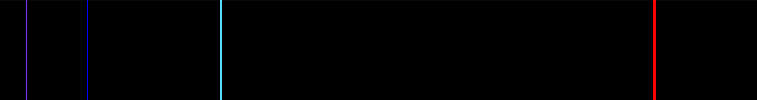
\includegraphics[width=0.7\linewidth]{files/Emission_spectrum-H-8dd91f1ad41c5b64ffa898637d5626f0.svg}
\caption[]{\textbf{Spectral lines.} Example diagram of the emission spectrum of Hydrogen (showing only lines in the visible part of the spectrum).}
\label{spectrum}
\end{figure}

In order to explain the existence of spectral lines from the perspective of classical physics, the small number of allowed frequencies of the emitted light must arise from some characteristic vibrations within the atom. But what could these characteristic vibrations be? Moreover, where does the intricate relation between the allowed wavelengths come from? Classical physics seems to provide no satisfactory answer to these questions, and therefore the existence of spectral lines was a mystery.

\subsubsection{The stability of the atom}\label{The stability of the atom}

A second problem concerns the stability of the atom. Once the nucleus and the electron had been discovered, one possible model for an atom was the `solar system' model, of a positively charged nucleus at the centre, around which the electron orbits.

Classical electromagnetism says however that \textbf{accelerating charges emit radiation}, and that this radiation carries away with it energy. The electron, which is undergoing circular motion, is accelerating constantly, and should therefore emit radiation and lose energy. Ultimately the electron should therefore spiral into the nucleus as it loses its energy and slows down.  Atoms in vacuum are however observed to be very stable, surviving almost indefinitely -- much longer than the timescale over which the electron should lose all its energy and spiral into the nucleus. No satisfactory way of accounting for the stability of atoms from such a classical model was ever found.

\subsubsection{Quantisation of angular momentum and the Bohr atom}\label{Quantisation of angular momentum and the Bohr atom}

Bohr was able to provide partial answers to both of these problems by postulating that \textbf{angular momentum of the electron is quantised}. In particular, Bohr postulated that much like the energy of a photon is quantised, so too is the angular momentum $L$ of an electron in orbit around a nucleus. Bohr postulated that an elementary \textbf{quanta} of orbital angular momentum is the \textbf{Reduced Plank constant}

This constant is commonly referred to simply as ''\textbf{h-bar}''. Bohr postulated that the angular momentum of electrons is only ever an integer multiple of $\hbar$, and no other value, $L = n\hbar$.

Under this assumption, Bohr was able to give a \textbf{stable} model for an atom. In particular, electrons do not radiate continuously as classical electromagnetism predicts, but lose angular momentum and energy in finite, quantised amounts, by emitting photons. This radiation continues until the electron has reached the minimum angular momentum of $\hbar$, after which it no longer radiates, and orbits the nucleus in a stable fashion. Bohr found that the radii and energies of the allowed orbits are

\begin{equation}
\label{e-Bohr-relations}
r_n = \frac{\epsilon_0 h^2 }{\pi M_e e^2}n^2,\quad E_n = -\frac{M_e e^4}{8 \epsilon_0^2 h^2} \frac{1}{n^2},
\end{equation}

where $\epsilon_0$ is the permittivity of free space, $M_e$ is the mass of the electron, $e$ is the electron charge, and $n$ is an arbitrary positive integer.

The spectral lines are also explained by this model. When an electron `jumps' from one orbit to another, its energy changes, and the photon carries away this energy. In particular, if it jumps from the orbit with energy $E_n$ to the one with energy $E_m$, then the photon must carry away the energy $\Delta E = E_m - E_n$.  However, Einstein already told us that a photon with energy $\Delta E$ has frequency $f = \Delta E/h$ and wavelength $\lambda = hc/\Delta E$. Thus

\begin{equation}
\frac{1}{\lambda} = \frac{\Delta E}{hc} = \frac{E_m - E_n}{hc} = \frac{M_e e^4}{8 \epsilon_0^2 h^3 c}\left(\frac{1}{n^2} - \frac{1}{m^2}\right).
\end{equation}

The constant out the front exactly matches the experimentally observed Rydberg constant, and thus reproduced the spectral lines of Hydrogen. In fact, this prediction of the Bohr model led to the search, and subsequent discovery of new lines outside the visible part of the electromagnetic spectrum, which had previously not been observed.

\subsection{Matter waves}\label{Matter waves}

Einstein postulated that electromagnetic radiation was in fact comprised of 'packets' which he called photons, which can roughly be thought of as particles. De Broglie postulated that \textbf{matter might conversely behave like a wave}. When electromagnetic radiation has energy $E$, its momentum is $p = E/c$. Using the Einstein formula for the energy of the photon, $E = hf = hc/\lambda$, we see that

\begin{equation}
p = \frac{E}{c} = \frac{hc}{\lambda c} = \frac{h}{\lambda}.
\end{equation}

De Broglie postulated that this formula \textbf{holds universally} for both radiation and matter, and prescribed that if a particle has momentum $p$ then it will behave like a wave of wavelength

At first sight this seems strange, but it can be readily seen that the wavelengths for ''everyday'' objects are so small that they would be imperceptible. However, for elementary particles, in conditions which could be formed in the laboratory at that time, in principle this wavelength should have been observable. Two-slit experiments were subsequently carried out, and interference effects, at the wavelength predicted by de Broglie, were observed, indicating that indeed matter can exhibit wave-like properties too.

However, this raised a huge number of questions. Were particles really waves? How does this fit with the conclusion of the photoelectric effect, that waves are in fact particles? There were numerous other phenomena that couldn't be explained -- subtle aspects of black-body radiation, the way x-rays scatter off solids, the so-called Compton effect. Everything pointed towards the need for a radical re-thinking of the physical world. Quantum mechanics was invented to answer these questions, and in the next section we will start of exploration of the basic aspects of this new theory.

\printbibliography

% DON'T EDIT. If "endfloat" option is enabled all floats appear before appendices
\if@endfloat\clearpage\processdelayedfloats\clearpage\fi


%%%%%%%%%%%%%%%%%%%%%%%%%%%%%%%%%%%%%%%%%%%%%%%%%%%%%%%%%%%%
%%% SUPPLEMENTARY MATERIAL / APPENDICES
%%%%%%%%%%%%%%%%%%%%%%%%%%%%%%%%%%%%%%%%%%%%%%%%%%%%%%%%%%%%
%% Sadly, we can't use floats in the appendix boxes. So they don't "float", but use \captionof{figure}{...} and \captionof{table}{...} to get them properly caption.

%%%%%%%%%%%%%%%%%%%%%%%%%%%%%%%%%%%%%%%%%%%%%%%%%%%%%%%%%%%%
%%% ARTICLE END
%%%%%%%%%%%%%%%%%%%%%%%%%%%%%%%%%%%%%%%%%%%%%%%%%%%%%%%%%%%%

\end{document}
